%source: path: /mnt/9636D17436D15639/University/Ta/Logic Design/Utils/Adel/EXAM/270EX2S22ans.pdf


ماژول وریلاگی به‌صورت رفتاری\footnote{\lr{Behavioral}} طراحی کنید که توصیف کننده مدار زیر باشد. ورودی این مدار، S و C و Clock است، همچنین خروجی آن X و Y است. کد شما باید درست، واضح و کوتاه باشد.

\begin{figure}[h]
	\centering
	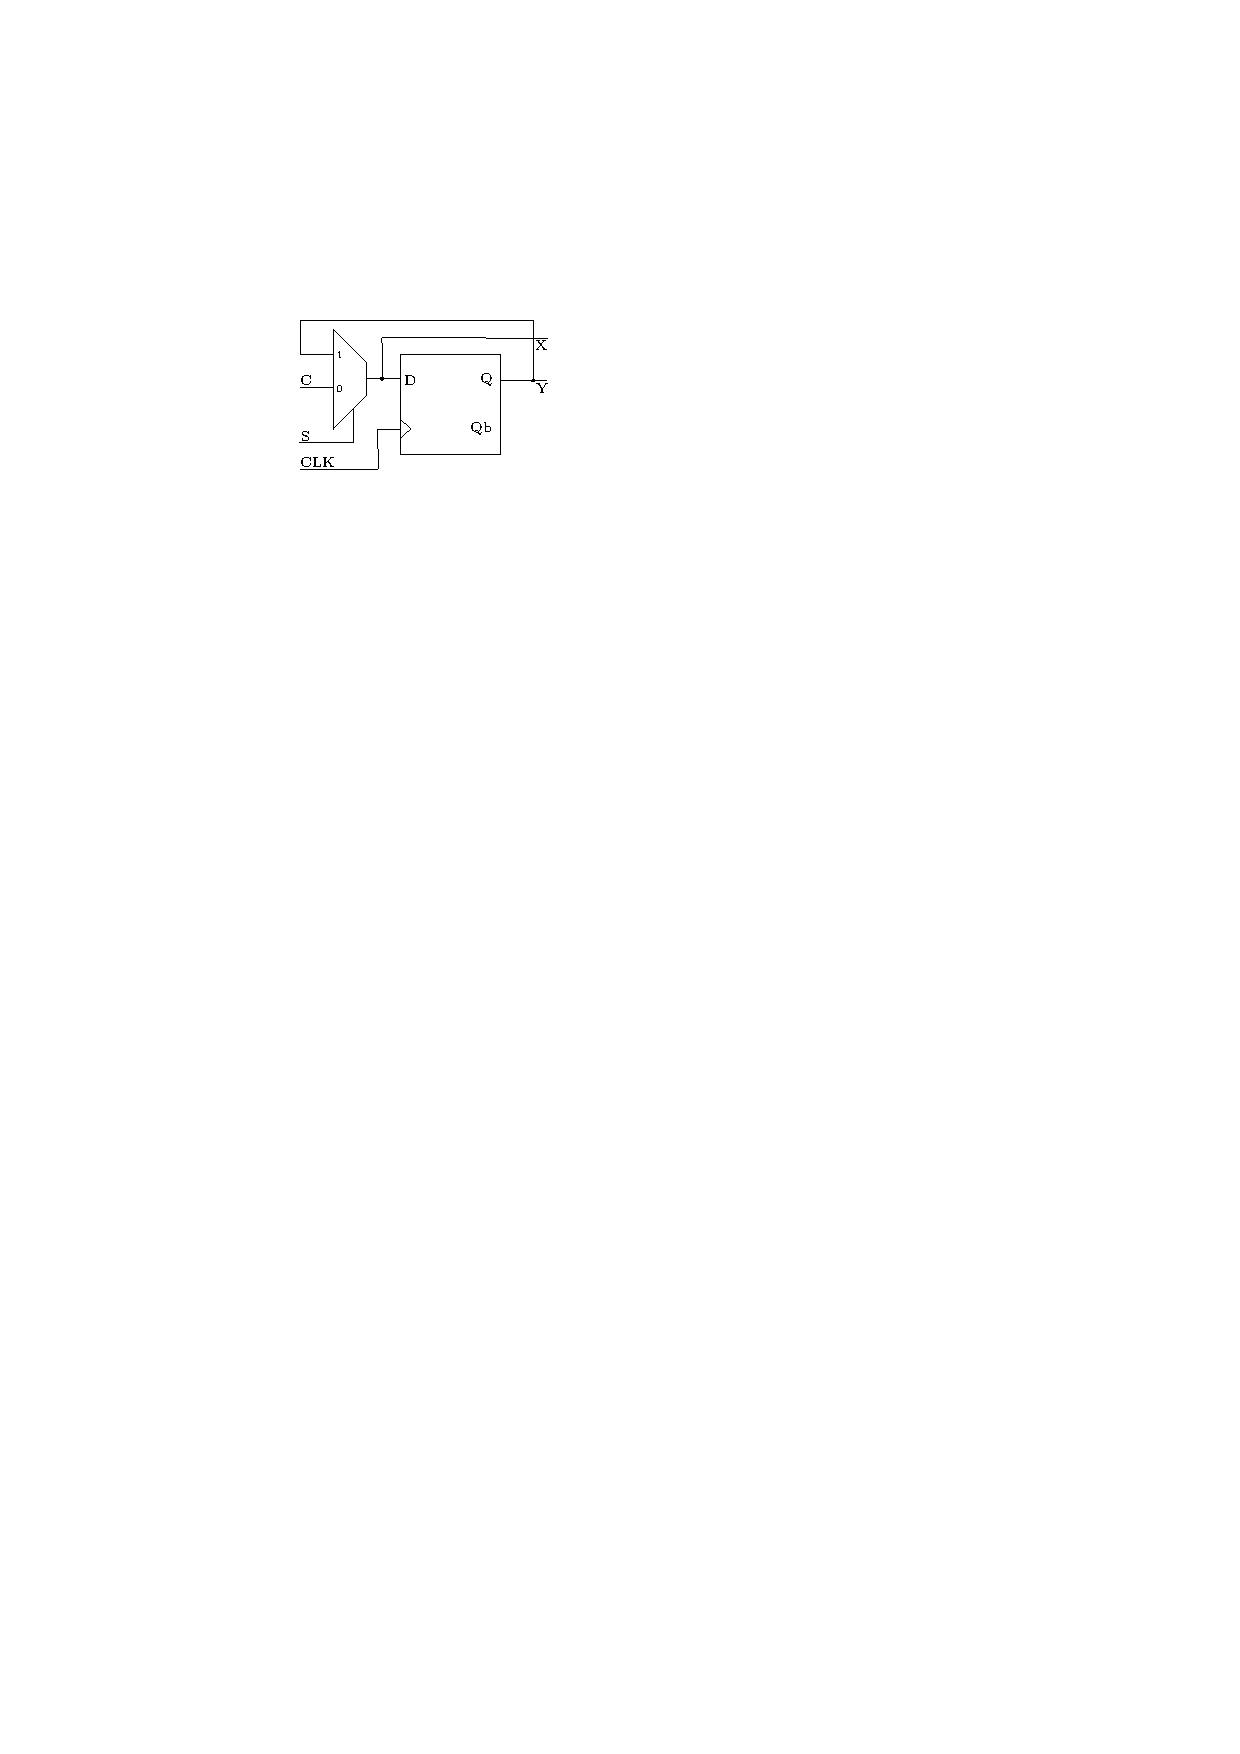
\includegraphics[width=0.4\textwidth]{fig/Q_bunos_2.pdf}
	\label{fig:Q_bunos_2}
\end{figure}

